%------------------------------------------------
% Request.tex
%
% This document build the incident frame
%------------------------------------------------
\section{Request Fulfillment}
\frame
{
\frametitle{Contenuti}
\tableofcontents[currentsection]
\addtocounter{framenumber}{-1}
}

\subsection*{Input e Output}
\begin{frame}{Input e Output}
\begin{table}
\begin{tabular}{ l | c }
\textbf{Input} & \textbf{Da}\\
\hline
RFC & Utenti\\
Notifiche & Change Management\\
\end{tabular}
\caption{Input di processo}
\end{table}
\begin{columns}
\begin{column}{0.3\textwidth}
\begin{figure}

\includegraphics[scale=0.1]{Images/Input_output.png}
\end{figure}
\end{column}
\begin{column}{0.7\textwidth}
\begin{table}
\begin{tabular}{ c | c }
\textbf{Output} & \textbf{Verso}\\
\hline
Notifiche & Utenti\\
\end{tabular}
\caption{Output di processo}
\end{table}
\end{column}
\end{columns}
\end{frame}

\subsection*{Metriche di processo}
\begin{frame}{Metriche}
Saranno prodotti report mensili con le seguenti metriche:
\begin{itemize}
\item{numero totale di richieste suddivise per tipo}
\item{tempo di risposta medio}
\item{tempo medio per completare le richieste}
\item{numero di richieste completate entro il relativo SLA}
\item{numero di carenze}
\end{itemize}
\begin{figure}
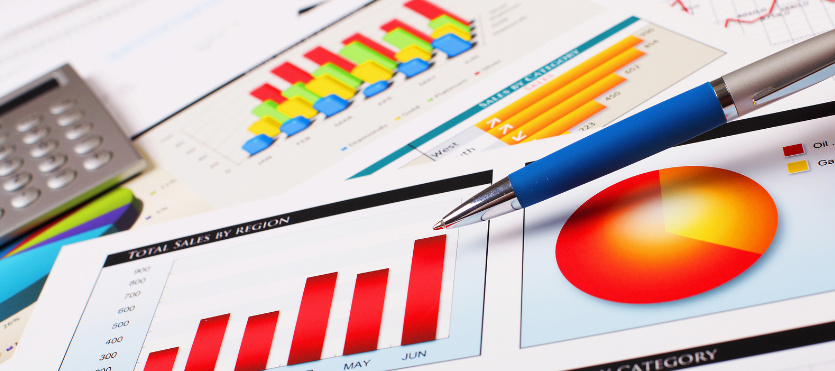
\includegraphics[scale=0.13]{Images/Metrics.png}
\end{figure}
\end{frame}

\subsection*{Attività di processo}
\begin{frame}{Attività di processo}
\begin{figure}
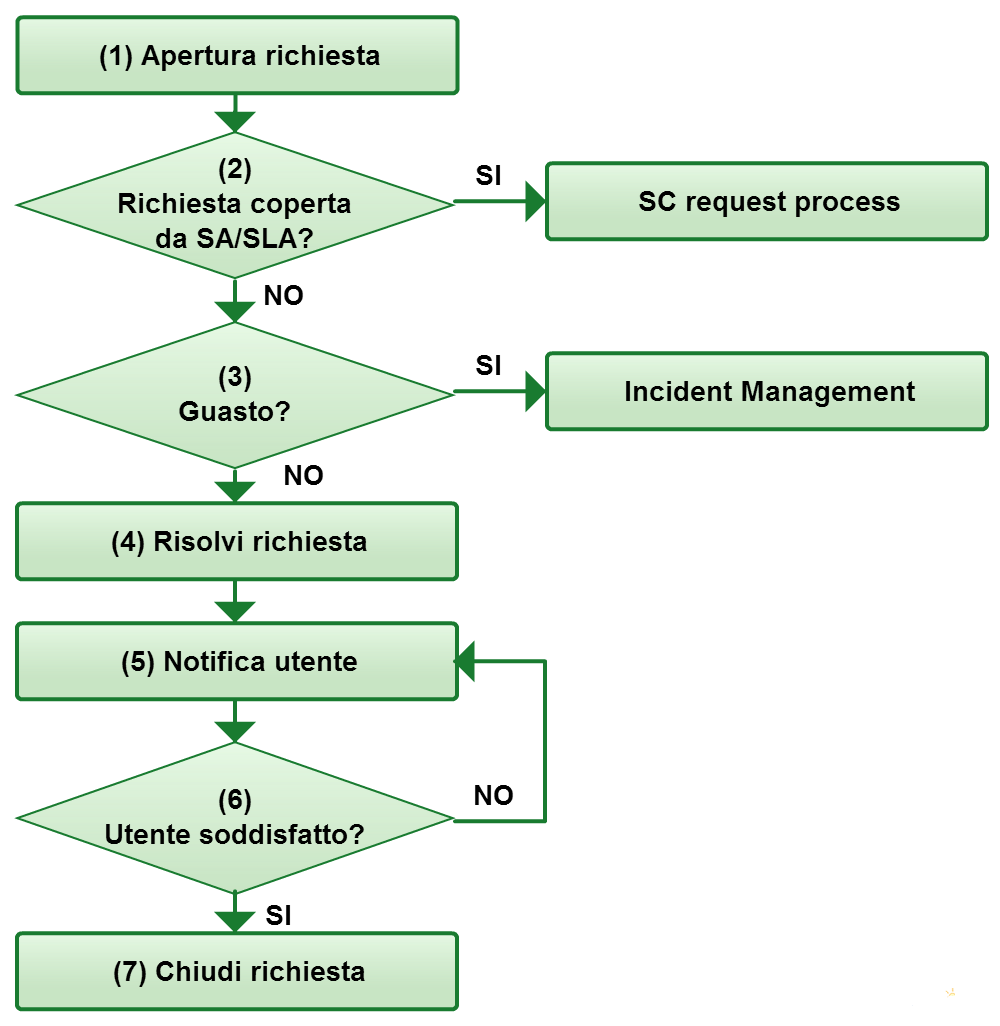
\includegraphics[scale=0.22]{Images/Request_fulfillment.png}
\end{figure}
\end{frame}